This chapter presents a survey of previously published related works that inform the design of a gesture authoring tool for skeletal tracking interfaces; in order to situate the work within the context of pertinent current research, reveal insights that may inform the design of the tool, and determine appropriate strategies for design and evaluation.

\section{Gestural Interaction}
\label{sec:gestural-interaction}

This section discusses dimensions that characterize gesture-based interactive systems and propose terms that clearly label pertinent concepts. Thus, the scope of and the design space for the research described in this thesis is partly situated in relation to previous works on gestural interaction.

Studies related to human gesture in HCI and IxD draw from a variety of domains, including but not limited to industrial design, psychology, anthropology, linguistics and computing. Here, also drawing from a multitude of disciplines, I argue that there are three important dimensions that characterize the design space for systems that utilize gesture as the main means of interaction (see Figure~\ref{fig:dimensions}):

\begin{enumerate}
\item The \emph{capture medium} is a high-level description of the hardware used to recognize gestures.
\item	The \emph{gestural bulk} is a description of the body parts involved in gesturing.
\item The gestural \emph{engagement domain} is a description the kinds of gesture that the system utilizes.
\end{enumerate}

\begin{SCfigure}[\sidecaptionrelwidth][b]
\centering
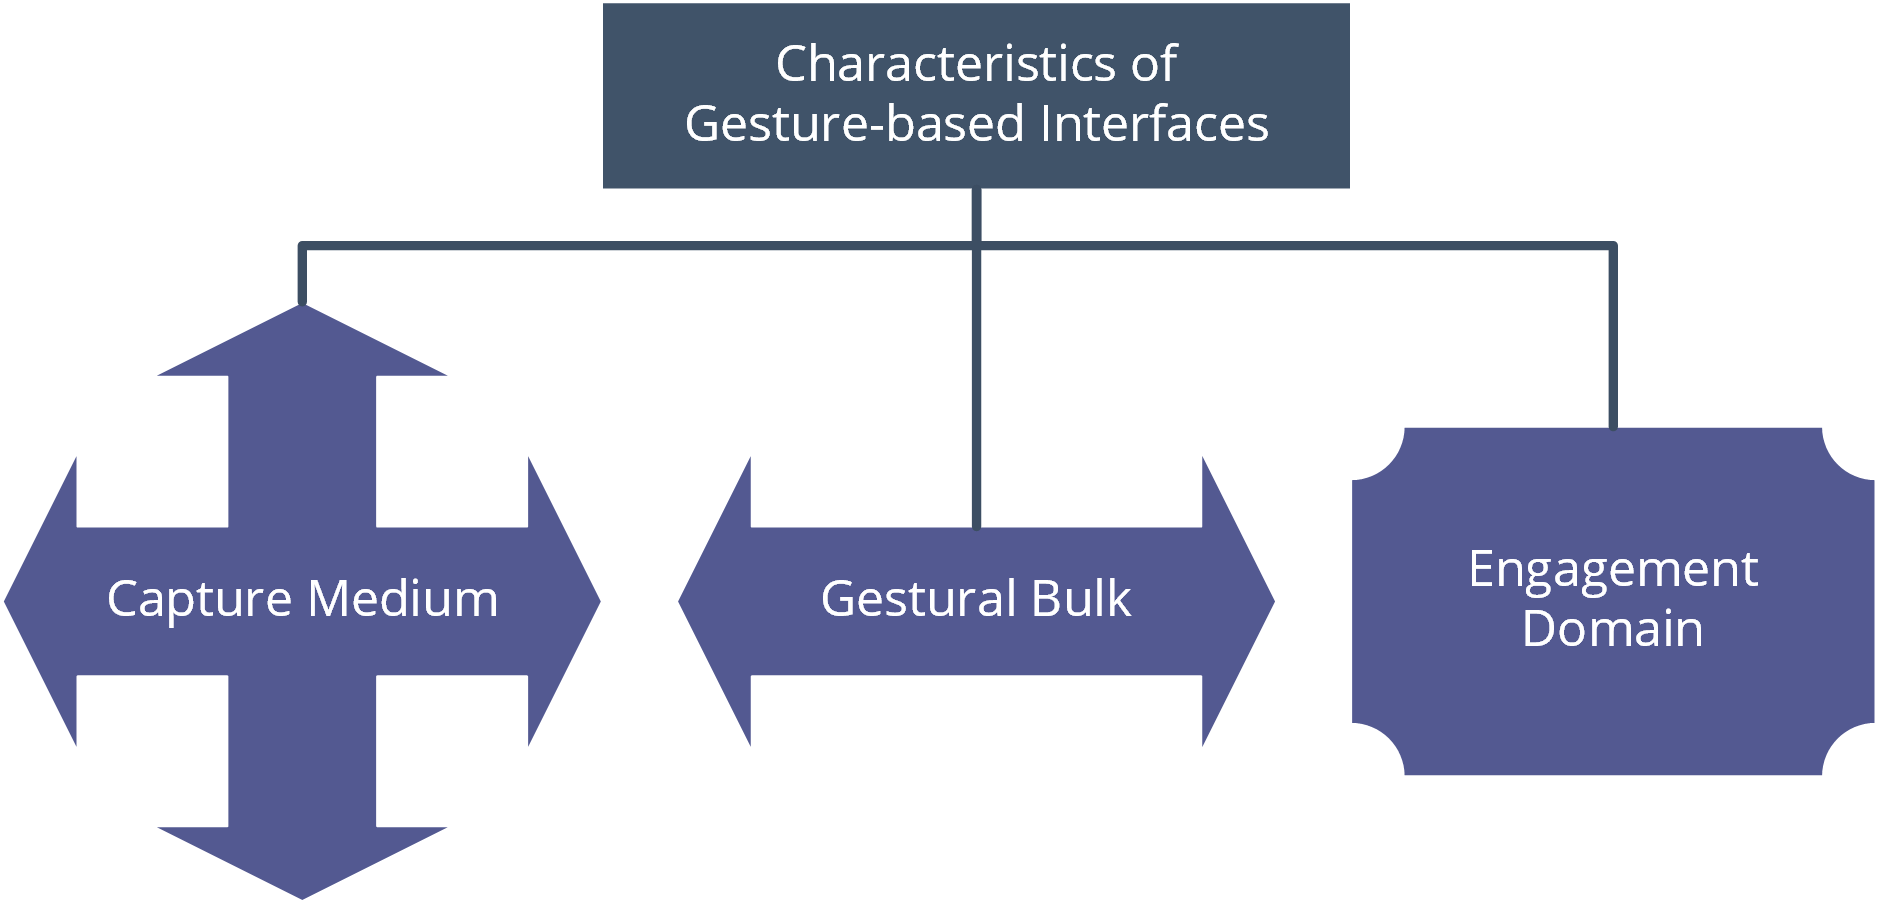
\includegraphics[width=0.6\textwidth]{dimensions}
\caption{Visualizing the three dimensions that characterize gesture-based interactive systems.}
\label{fig:dimensions}
\end{SCfigure}

\clearpage

The first of these dimensions, the \emph{capture medium}, describes the hardware technology used for sensing gestures. The hardware in this sense may comprise a 2-dimensional space that allows gesturing with a tangible pointing device such as a mouse or pen or a surface that detects touch events without utilizing a pointing device; tangible sensors that detect gestures in 3D space; perceptual input devices that “see” human movement from a distance; or myriad other current and emerging technologies (Figure~~\ref{fig:capture-media}).

Capture media differ in accordance to the degrees of freedom of the space in which the gestures are performed. It should be noted that while the degrees of freedom of the performance space is related to the degrees of freedom that the hardware can sense, the two are not the same: For instance, when gesture sensing is performed using cameras with algorithms based on edge detection instead of depth sensing \parencite{Moeslund:2001, Moeslund:2006}; computers are often only able to recognize activity in the horizontal and vertical, while changes in depth are ignored. However, from the user’s perspective, the gestures are performed on a 3-dimensional medium, regardless of the level of detail that the computer can sense.

Adopting the user’s perspective, I distinguish between \emph{free-form} and \emph{constrained} capture media. I propose term \emph{constrained} to identify capture media where gestures are performed on a 2-dimensional surface, while the term \emph{free-form} identifies capture media where gestures are performed in a 3-dimensional volume. Examples to constrained capture media are computer mice, trackpads and touchscreens; while camera- and accelerometer-based gesture sensing systems constitute examples to free-form capture media.

Capture media also differ according to whether or not they require special input devices to be worn or wielded by the user. An input device in this sense denotes any electronic device or object that is directly coupled to the movement or position of the body part(s) that make up the gesture. In most cases where such input devices are used, the system senses only the movements or the position of the input device. \textcite{Quek:1996} has previously coined the term \emph{unencumbered} to describe a class of capture media that do not employ such devices. The term has been used previously to refer only to \emph{free-form} interactions. I wish to extend its definition to also accommodate \emph{constrained} capture media that do not require pointing devices be used on the gesture-sensing surface, e.g. touchscreens that can be manipulated by human fingers alone.  Conversely, when the capture medium --– whether \emph{constrained} or \emph{free-form} –-- relies on input devices such as mice, styli, gloves or accelerometers; I propose the term \emph{equipped} to describe it.

A device that allows gestural interaction does not need to afford only one capture medium. Indeed, modern smartphones offer touchscreens that allow for both equipped and unencumbered input, while they also function as equipped free-form capture media since they harbor accelerometers and gyroscopes.

\begin{SCfigure}[\sidecaptionrelwidth][t]
\centering
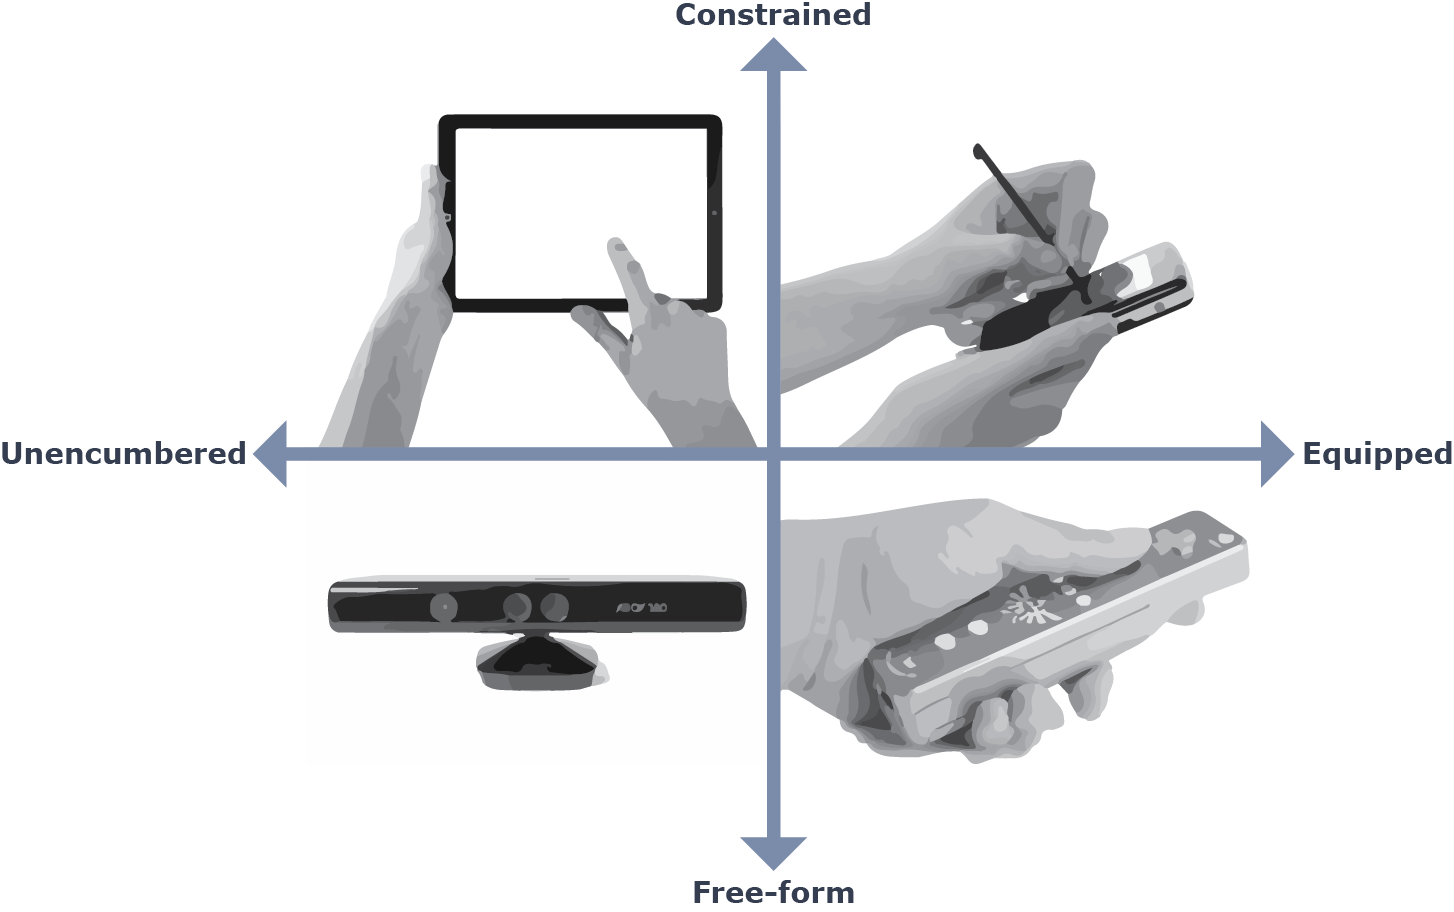
\includegraphics[width=0.7\textwidth]{capture-media}
\caption{Classifying capture media. A capture medium can be \emph{constrained} or \emph{free-form} depending on the space where gestures are performed, and \emph{unencumbered} or \emph{equipped} depending on the use or non-use of an input device that proxies human movement.}
\label{fig:capture-media}
\end{SCfigure}

The second dimension, the \emph{gestural bulk} describes body parts involved in interacting with the system. Following conventional terminology in kinesiology; I classify gestures for HCI as those relying on \emph{fine motor movements}  and those that rely on \emph{gross motor movements}. \emph{Fine movements} are precise and involve small musculature; e.g. typing on a keyboard or writing with a pen. \emph{Gross movements} require the use of larger muscles and emphasize muscular force over precision; e.g. jumping or weight lifting. Section~\ref{sec:scope} describes this dimension in greater detail, in order to clarify the scope of my research.

The last of the dimensions I propose to classify gesture-based interactive computing systems is the gestural \emph{engagement domain}, which describes what kinds of gestures a user interface utilizes. Psychology \parencite{McNeill:1992, McNeill:2008} often provides the basis for classifications and analyses of human gesture in HCI and IxD literature\footnote{In computing, the term \emph{classification} also refers to the outcomes from a machine learning algorithm. Here, I use the term in pertinence to the characterization of gestures.} \parencite{Eisenstein:2006, Kettebekov:2004, Wexelblat:1997}. The perspective on the classification of human gestures proposed by \textcite{Quek:2002} and extended by \textcite{Karam:2005} draws from these studies and forms an appropriate basis for my classification, albeit with modifications. I distinguish human gestures as belonging to one of four classes:

\begin{enumerate}
\item \emph{Deictic gestures} that involve pointing to convey the identity and/or position of an entity.
\item \emph{Manipulative gestures} that involve a direct connection between movements and the properties of an entity in the system in use.
\item \emph{Semaphoric gestures} that function as symbols attached to a clear meaning.
\item \emph{Gesticulations} that accompany speech.
\end{enumerate}

\emph{Deictic gestures} involve pointing (often with hands and/or fingers) to communicate the identity and/or the position of an entity. The canonical example for the use of deictic gestures in computing applications was implemented in MIT‘s “Media Room,” where free-form pointing at items on a computer screen while uttering verbs and pronouns was exploited as an interface modality \parencite{Bolt:1980}. Somewhat unconventionally, since I adopt a broad definition for what \emph{gesture} denotes, what I label as deictic gestures also includes everyday interactions such as pointing and clicking with a mouse or pressing a button on a touchscreen.

\emph{Manipulative gestures} correspond to situations where "a tight relationship between the actual movements of the gesturing hand/arm with the entity being manipulated" is established \parencite{Quek:2002}. Using such gestures, often on \emph{constrained capture media}, for moving, resizing and otherwise transforming objects on a display are common in contemporary desktop and mobile computing scenarios. Examples for manipulative gestures on constrained capture media include actions such as “drag-and-drop,” drawing a box with the mouse cursor to select multiple items on the screen, and touch-scrolling documents on a touchscreen tablet. On free-form capture media; the primary interactions in sports games such as bowling or tennis on the Nintendo Wii constitute examples for manipulative gestures: The movements of the handheld controller are tightly related to the movements of a ball, a racquet, a sword etc.

\emph{Semaphoric gestures} --- also referred to as "emblems" \textcite{McNeill:2008} --- are static poses or dynamic movements that function as symbols attached to a clear meaning. Sign language gestures --- which some researchers such as \textcite{McNeill:2008}; and textcite{Karam:2005} consider to be distinct from semaphores --- may be considered semaphoric to the extent that they relate to my analysis. Examples for semaphoric gestures commonly used in computing include the mouse-controlled “navigation gestures” implemented in version 11 of the Opera web browser and the “wave to engage” gesture that proposed in Microsoft's 2013 \emph{Kinect for Windows Human Interface Guidelines}.
Although demonstrated in many works \parencite{Cao:2003, Lenman:2002, Wilson:2003}; \textcite{Wexelblat:1995} disputes the usefulness of strictly semaphoric gestures in HCI, with the argument that "the one-to-one mapping of input to command reduces gesture to only the expressive power of a function-key pad." However, recent sensing technologies and implementation aides allow for very rapid development of interactions that employ semaphoric gestures. This leads to a proliferation of content that exploits the limited expressive power of semaphores for meaningful use. Today, in many cases, the use of semaphoric gestures over a key pad makes sense when aspects such as the system's cost and context, pedagogical considerations, and/or the overall user experience \parencite{Fogtmann:2008} are taken into account.

The final class of gestures that is relevant for HCI and IxD are \emph{gesticulations}, which comprise what \textcite{McNeill:2008} calls "motion that embodies a meaning relatable to the accompanying speech" --– i.e. body movements produced along with speech to clarify or augment its content. The recognition of gesticulations is an important technical challenge in computing. The most common applications for gesticulations in HCI are affect recognition and multimodal interfaces where they accompany a speech recognition system to remove ambiguity and extend the interactive capacity \parencite{Kopp:2004, Krum:2002, Silva:2003}.

There are, of course, gestures that do not fall strictly into one of the categories above. A swipe towards the left on a trackpad or tablet that is commonly utilized to invoke a “go back” command, for example, may be classified as a manipulative as well as a semaphoric gesture depending on the context and the system’s feedback. However, I find this classification to be relevant and useful for examining gesture-based interfaces for what sort of gestural triggers they implement; hence specifying which domain of gestures that such interfaces can engage.

Some of the terms and concepts I propose are, to my knowledge, novel; and I believe they will foster future research and discussion: The distinction of \emph{constrained} vs. \emph{free-form} and \emph{equipped} vs. \emph{unencumbered} \emph{capture media} will come in handy for classifying works appropriately. Yet, gesture-based HCI is a rapidly advancing field, with new technologies and concepts being introduced continuously. Thus, I am not putting forward an exhaustive and conclusive treatment of the topic. I covered what I believe are the most salient characteristics of gesture-based interactive systems and compiled a set of terms and concepts to support discussion and situation of my work.

In terms of the concepts introduced in this section, the \hl{scope} of this thesis pertains to the design of a gesture authoring tool for use with \hl{\emph{perceptual}} (\emph{unencumbered, free-form}) input devices that sense \hl{\emph{gross} gestures.} In line with the desiderata uncovered through formative studies (see Section~\ref{sec:formative-studies}), the gestural \hl{\emph{engagement domain}} that influences the expressive power of the resulting authoring tool is limited to \hl{\emph{semaphoric gestures}}, although support for \emph{deictic} and \emph{manipulative} gestures can be "hacked" together using various strategies (see Chapter~\ref{chp:hotspotizer}).

\section{End-User Programming}
\label{sec:end-user-programming}

"Programming" can be defined as "the process of transforming a mental plan of desired actions for a computer into a representation that can be understood by the computer" \parencite{Myers:2006}. The study of various aspects of programming has been a long-established topic of human-computer interaction research. Traditionally, the focus of this field has been on the activities of professional programmers and novices who are aiming to become professionals. A relatively recent topic of interest is the study of end-user programming as a topic distinct from the activities of professional and novice software developers \parencite{Myers:2006}. As such, interaction with a diverse array of devices --- e.g. TVs, telephones, alarm clocks... --- and a diverse assortment of tasks comprise topics of interest for programming research.

What differentiates an end-user from a professional programmer is their \emph{goals}: Professionals create and maintain software as an end, while end-users produce and customize software artifacts to support their own goals in some other domain \parencite{Ko:2011}. In many domains, the case for end-user programming --- rather than entrusting all development to professionals --- is mainly economical:  \textcite{Wulf:2004} argue that support for end-user programming makes software investments more efficient since empowering end-users to customize software mitigates the need for expensive development teams and processes (see Figure~\ref{fig:eud}). The effect is significant, since end-users outnumber professional programmers by orders of magnitude \parencite{Scaffidi:2005}. From a user-focused perspective, research on end-user programming is motivated by usability and engagement concerns \parencite{Germonprez:2007}; as well as the simple fact that some systems such as smart homes \parencite{Blackwell:2004} and health-related applications \parencite{Rizzo:2011, Lange:2011} must be customizable to suit individual needs \parencite{Holloway:2010}.

\begin{SCfigure}[\sidecaptionrelwidth][t]
\centering
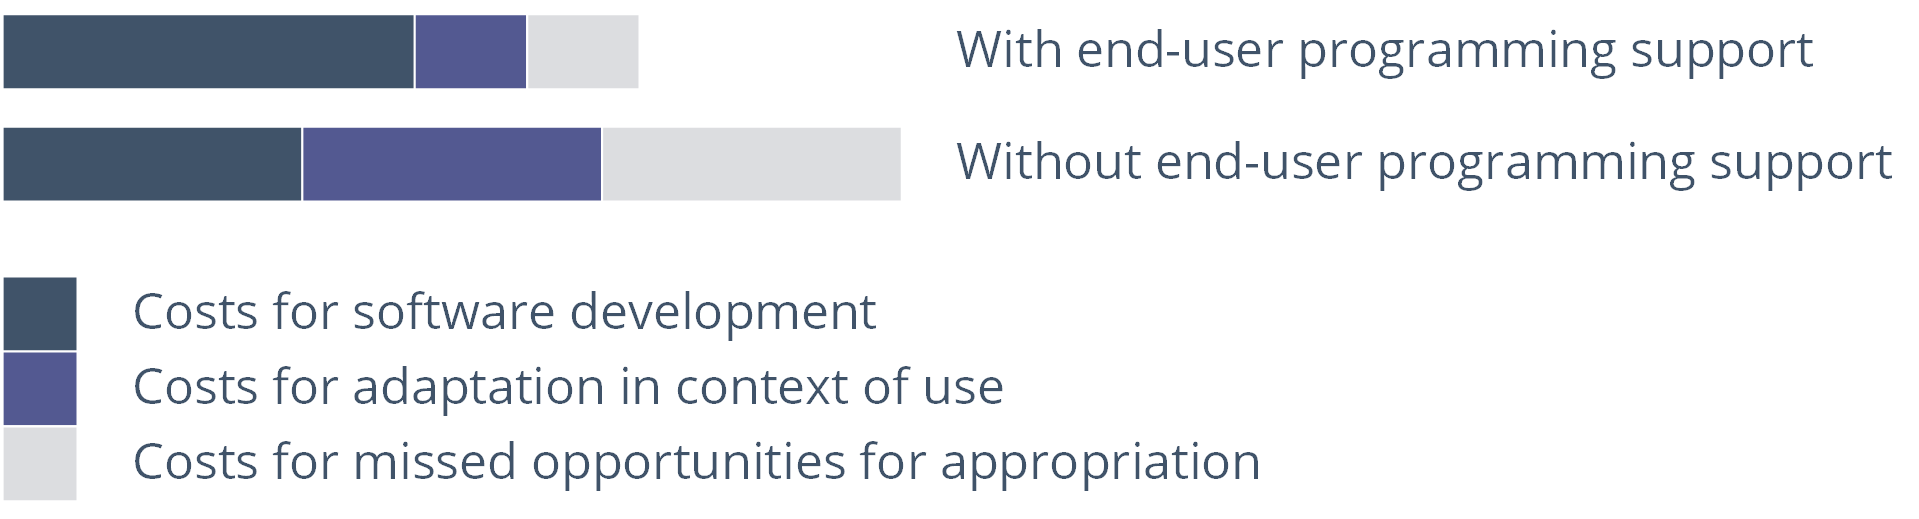
\includegraphics[width=0.7\textwidth]{eud}
\caption{Comparing the cost structure for software development, adaptation and appropriation with and without end-user programming support. Adapted from \textcite{Wulf:2004}.}
\label{fig:eud}
\end{SCfigure}

This thesis covers the design and development of a gesture authoring tool for designers' prototyping novel user interfaces and end-users' extending existing interfaces with the ability to recognize and respond to custom mid-air gestures. Various works on end-user programming that inform this effort are discussed below. A complete survey of this field is beyond the scope of this work; I recommend surveys by \textcite{Paterno:2013}; and \textcite{Myers:2006} as a starting point for the interested reader.

One strand of research on end-user programming considers issues beyond the construction and customization of software; e.g. design, testing, debugging, integration, reuse, and security. This strand, called \emph{end-user software engineering}, aims improve the \emph{quality} of software artifacts produced by end-users by leveraging knowledge derived from professional software engineering. A comprehensive review of this research is beyond the scope of this thesis. While end-users' design, specification, testing, debugging, and reuse of software artifacts are indeed relevant for a gesture authoring tool; this thesis  (as Chapter~\ref{chp:design} describes) approaches such issues from a \hl{design --- rather than software engineering --- perspective.} For the reader interested in end-user software engineering, I recommend surveys by \textcite{Burnett:2004}, and \textcite{Ko:2011}.

A number of end-user programming researchers focus on psychological and cognitive issues that relate to end-user programmers. One objective for such research, as \textcite{Blackwell:2006} declares in his survey of the field, is "to increase our understanding of human cognition by studying a rather extreme domain of reasoning." Another objective is to tackle quality issues by informing the design of end-user programming tools and methods. Topics of interest include the difficulties of learning \parencite{Ko:2004, Pea:1987} and performing \parencite{Lewis:1987} programming-related tasks, and how people envision programming concepts \parencite{Pane:2001}.

From among research on the psychology of programming, particularly relevant for a gesture authoring tool is work by \textcite{Ko:2004} where the authors identify six "learning barriers" that obstruct end-user programmers across a variety of contexts:

\clearpage

\begin{enumerate}
\item \emph{Design barriers} are difficulties that are inherent in a problem, independent from how the solution is represented. They represent the inability of a learner to construct a solution to a given problem, which must be accomplished before the solution is implemented as software.
\item \emph{Selection barriers} impede learners from discovering what components are afforded by the programming environment, and which of those can be used to implement their design for a software solution.
\item \emph{Coordination barriers} hinder learners' understanding of how various components offered by the programming environment can be combined to achieve desired behaviors.
\item \emph{Use barriers} obscure the intent, usage and effects of programming components. To illustrate with an example: a learner may have determined that they need to use a "list" structure to implement an algorithm, but they may not know how to declare and initialize one within the programming environment.
\item \emph{Understanding barriers} arise when learners are not able to compare the external behavior, i.e. the results, of the software with their expectations. This is usually a result of an absence or inadequacy of feedback as to what the software does or does not do.
\item \emph{Information barriers} disrupt learners' understanding of the internal workings of the software. They manifest as learners' inability to test hypotheses they might have about how the software does what it does.
\end{enumerate}

The authors relate these learning barriers to \posscite{Norman:1986, Norman:2002} concepts of the \emph{gulf of execution} and the \emph{gulf of evaluation} (which I described in section~\ref{sec:motivation} to motivate the development of a gesture authoring tool). Specifically, they explicate that \emph{design}, \emph{coordination}, and \emph{use} barriers spawn gulfs of \emph{execution}; \emph{understanding} barriers pose gulfs of \emph{evaluation}; while \emph{selection} and \emph{information} barriers constitute gulfs of \emph{execution} and \emph{evaluation}. The authors recommend adapting \posscite{Norman:1986, Norman:2002} recommendations for bridging the gulfs and overcoming the learning barriers.

\section{Design and Evaluation of User Interface Authoring Tools}
\label{sec:design-and-evaluation-of-tools}

\textcite{Olsen:2007} argues that user interface design tools, particularly those that deal with unconventional interaction techniques (e.g. mid-air gesture sensing), do not lend themselves to conventional software evaluation methods. One reason for this is that such tools require domain-specific expertise, which --- by the nature of novel tools --- no user population possesses. Another reason is that these tools support complex tasks with high inter-user variability in terms of the users’ mental models of the tasks. “Meaningful comparisons between two tools for a realistically complex problem are confounded in so many ways as to make statistical comparisons more fantasy than fact.” \parencite{Olsen:2007} From the framework proposed by Olsen for the evaluation of user interface toolkits, I derived the following four guidelines to direct the design of my mid-air gesture authoring tool:

\begin{itemize}
\item \emph{Reduce development time.} A good authoring tool should allow for the rapid implementation of design changes. This can be encouraged by reducing the number of choices that have to be made to express a design. (Granted, there may exist a tradeoff between this concern and the expressive power of the authoring tool.)
\item \emph{Encapsulate and simplify expertise.} Considerable technical know-how is required to design and develop applications for emerging technologies. A good design tool liberates the designer from the need for prior knowledge, yet communicates the capabilities and limitations of the technology to nudge the designer towards feasible designs.
\item \emph{Lower skill barriers.} Empowering new populations of users to envision and implement designs “expands the set of people who can effectively create new applications.” \parencite{Olsen:2007}
\item \emph{Make use of a common infrastructure.} It is difficult to get users to adopt a new standard. As much as possible, authoring tools should hook up to existing and widely adopted tools and practices, and complement existing workflows; upgrading rather than negating the common denominator.
\end{itemize}

Employing a user interface paradigm for expressing design choices that reflects the problem being solved and embodies the constraints of the design space \parencite{Norman:1993} serves all four the guidelines above.

In addition, \textcite{Shoemaker:2010} propose design guidelines for body-centric interaction with large displays. From among the guidelines they propose, two generalize to influence the design of an authoring tool for mid-air gestures:

\begin{itemize}
\item Interaction using mid-air gestures at a distance should be \emph{“mediated through a representation that binds personal and extrapersonal space.”} A means for communicating the constraints and opportunities of the interaction space to the user is recommended for mid-air gestural interfaces. This holds for design tools that target these interactions.
\item It is recommended that \emph{users’ sense of proprioception be leveraged} by allowing some operations to be performed in the user’s personal space, without requiring visual feedback. In terms of authoring interactions, this guideline calls for encouraging gesture designs that capitalize on proprioception through the nature of the authoring paradigm.
\end{itemize}

In sum, \hl{six guidelines derived from previous work form the basis of my design rationale} for the gesture authoring interface (Figure~\ref{fig:design-guidelines}). The first four, derived from \posscite{Olsen:2007} work, identify and address concerns that pertain to user interface design tools. The last two, derived from the work of \textcite{Shoemaker:2010}, attend to concerns related to perceptual interactions in general. Whether or not the final design for the authoring tool conforms to these guidelines is evaluated through user studies.

\begin{SCfigure}[\sidecaptionrelwidth][b]
\centering
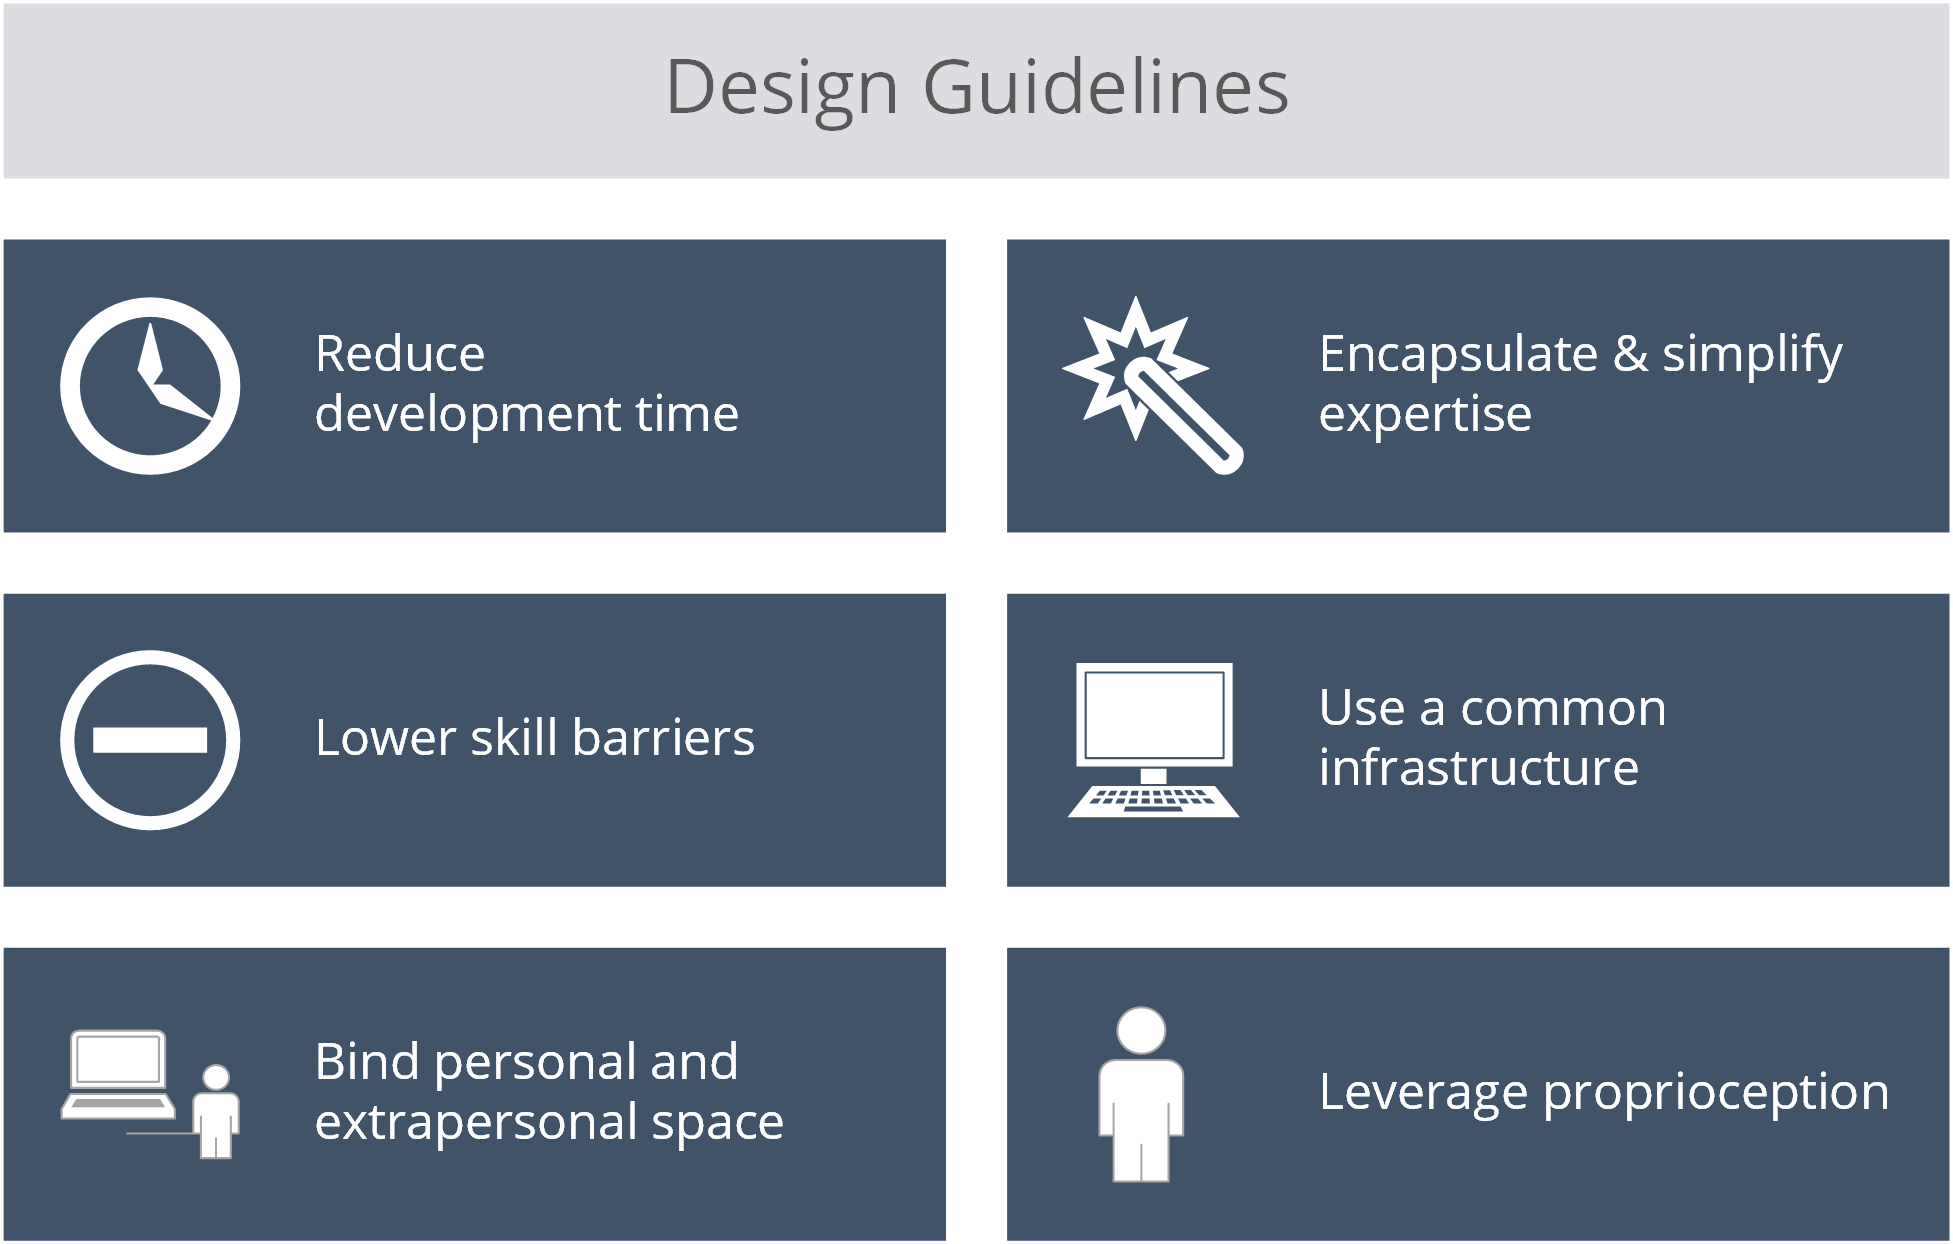
\includegraphics[width=0.7\textwidth]{design-guidelines}
\caption{Guidelines derived from the literature formed the basis of the design rationale for a gesture authoring tool.}
\label{fig:design-guidelines}
\end{SCfigure}

\clearpage

Additionally, from a programming perspective (see Section~\ref{sec:end-user-programming}), \textcite{Myers:2000} identify five themes that influence the success of user interface tools:

\begin{itemize}
\item User interface tools should strive to achieve a low \emph{threshold} --- i.e. be easy to learn --- and a high \emph{ceiling} --- i.e. significant expressive power.
\item Successful tools lead users to making the right choices and avoiding wrong designs by offering a well-designed \emph{path of least resistance}
\item A tool should embody \emph{predictability} and avoid unpredictable automatic operations.
\item Developers of user interface tools should stay on top of developments, since user interface technologies are \emph{moving targets} that can change significantly or become obsolete at a rapid pace.
\item A tool should only \emph{address the parts of the user interface that are needed}.
\end{itemize}

The first of these themes is specifically captured in part by Olsen's recommendations that a tool should lower skill barriers and empower new users. A high level of expressive power is desirable, but the weight of this concern will be governed by user needs (see Section~\ref{sec:formative-studies}). The encapsulation and simplification of expertise, along with the use of user-centered design tools and methods, integrate all of these themes.

\section{Authoring Mid-Air Gestures}
\label{sec:authoring-mid-air-gestures}

This section presents an overview of prior research on gesture authoring tools which has influenced my design. While development tools provided by vendors of gesture-sensing hardware focus on supporting textual programming, ongoing research suggests a set of diverse approaches to the problem of how to represent and manipulate three-dimensional gesture data. Existing works approach the issue in three ways that constitute distinct paradigms for visually authoring mid-air gestures. These are:

\begin{enumerate}
\item using 2-dimensional graphs of the data from the sensors that detect movement;
\item using a visual markup language; and,
\item representing movement information using a timeline of
frames.
\end{enumerate}

In addition, there are approaches to manipulating gesture information that rely predominantly on textual representations.

These paradigms for visualizing and manipulating gesture data often interact with two approaches to authoring gesture information:

\begin{itemize}
\item Authoring gestures by \emph{declaration} involves the use of a high-level syntax to describe gesture information without specifying a computational control flow.
\item Authoring gestures by \emph{demonstration} is done by recording one or more examples and employing machine learning techniques to train a recognizer.
\end{itemize}

In addition, gestures can be defined through \emph{imperative} programming, in terms of a sequence of states or actions. This is the standard approach for authoring gestures in general-purpose textual programming environments. From a design perspective, this approach embodies significant gulfs of execution and evaluation, while erecting learning barriers for end-users (see Sections~\ref{sec:motivation}~and~\ref{sec:end-user-programming}). Imperative authoring of gestures is also suboptimal from a software engineering perspective (see Section~\ref{sec:motivation}; as well as \textcite{Hoste:2014}). Thus, imperative textual programming has not influenced my design significantly.

The three visual authoring paradigms enumerated above do not have to be used exclusively, and nor do demonstration and declarative programming. Aspects of different paradigms may find their place within the same user interface. A popular approach, for example, is to introduce gestures by demonstration, convert gesture data into a visual representation, and then declaratively modify it.

Below, I use examples from the literature to elaborate on the approaches enumerated above. I comment on their strengths and weaknesses based on previously published evaluations conducted with software that implement them.

Some of the work discussed below pertains to gesture-sensing systems which employ intrusive methods (e.g. markers or inertial sensors) rather than perceptual input devices. Even though the scope of this thesis does not fully encompass the intrusive sensing of mid-air gestures; the user interfaces of gesture authoring applications for intrusive sensors have aspects that inform the design of an authoring tool for perceptual interfaces. Thus, tools that target intrusive sensing applications and tools for perceptual interfaces are both considered.

\subsection{Using Graphs of Movement Data}

Visualizing and manipulating movement data using 2-dimensional graphs that represent low-level kinematic information is a popular approach for authoring mid-air gestures. This approach is often preferred when gesture detection is performed using inertial sensors such as accelerometers and gyroscopes. It also accommodates other sensors that read continuously variable data such as bending, light and pressure. Commonly the horizontal axis of the graph represents time while the vertical axis corresponds to the reading from the sensor. Often a “multi-waveform” occupies the graph, in order to represent data coming in from multiple axes of the sensor. Below, we study three software tools that implement graphs for representing gesture data: \emph{Exemplar}, \emph{MAGIC} and \emph{GIDE}.

\subsubsection{Exemplar}

\emph{Exemplar} \parencite{Hartmann:2007} relies on \emph{demonstration} to acquire gesture data and from a variety of sensors - accelerometers, switches, light sensors, bend sensors, pressure sensors and joysticks. Once a signal is acquired via demonstration, on the resulting graph, the developer marks the area of interest that corresponds to the desired gesture. The developer may interactively apply filters on the signal for offset, scaling, smoothing and first-order differentiation. \emph{Exemplar} offers two methods for recognition: One is pattern matching, where the developer introduces many examples of a gesture using the aforementioned method and new input is compared to the examples. The other is thresholding, where the developer manually introduces thresholds on the raw or filtered graph and gestures are recognized when motion data falls between the thresholds. This type of thresholding also supports hysteresis, where the developer introduces multiple thresholds that must be crossed for a gesture to be registered.

\emph{Exemplar}’s user studies suggest that this implementation of the paradigm is successful in increasing developer engagement with the workings and limitations of the sensors used. Possible areas of improvement include a technique to visualize multiple sensor visualizations and events and finer control over timing for pattern matching.

\subsubsection{MAGIC}

\posscite{Ashbrook:2010} \emph{System for Multiple Action Gesture Interface Creation (MAGIC)} is another tool that implements the 2-dimensional graphing paradigm. The focus of \emph{MAGIC} is programming by \emph{demonstration}. It supports the creation of training sets with multiple examples of the same gesture. It allows the developer to that keep track of the internal consistency of the provided training set; and check against conflicts with other gestures in the vocabulary and an “Everyday Gesture Library” of unintentional, automatic gestures that users perform during daily activities. \emph{MAGIC} uses the graph paradigm only to visualize gesture data and does not support manipulation on the graph.

One important feature in \emph{MAGIC} is that the motion data graph may be augmented by a video of the gesture example being performed. Results from user studies indicate that this feature has been highly favored by users, during both gesture recording and retrospection. Interestingly, it is reported that the “least-used visualization [in \emph{MAGIC}] was the recorded accelerometer graph;” with most users being “unable to connect the shape of the three lines [that correspond to the 3 axes of the accelerometer reading] to the arm and wrist movements that produced them.” Features preferred by developers turned out to be the videos, “goodness” scores assigned to each gesture according to how they match gestures in and not in their own class, and a sorted list depicting the “distance” of a selected example to every other example.

\subsubsection{GIDE}

\emph{Gesture Interaction Designer (GIDE)} by \textcite{Zamborlin:2014} features an implementation of the graph paradigm for authoring accelerometer-based mid-air gestures. \emph{GIDE} leverages a “modified” hidden Markov model approach to learn from a single example for each gesture in the vocabulary. The user interface implements two distinct features: (1) Each gesture in the vocabulary is housed in a “gesture editor” component which contains the sensor waveform, a video of the gesture being performed, an audio waveform recorded during the performance, and other information related to the gesture. (2) A “follow” mode allows the developer to perform gestures and get real- time feedback on the system’s estimate of which gesture is being performed (via transparency and color) and where they are within that gesture. This feedback on the temporal position within a gesture is multimodal: The sensor multi-waveform, the video and the audio waveform from the video are aligned and follow the gestural input. \emph{GIDE} also supports “batch testing” by recording a continuous performance of multiple gestures and running it against the whole vocabulary to check if the correct gestures are recognized at the correct times.

User studies on \emph{GIDE} reveal that the combination of multi- waveform, video and audio was useful in making sense of gesture data. Video was favored particularly since it allows developers to still remember the gestures they recorded after an extended period of not working on the gesture vocabulary. Another finding from the user studies was the suggestion that the “batch testing” feature where the developer records a continuous flow of many gestures to test against could be leveraged as a design strategy --- gestures could be extracted from a recorded performance of continuous movement.

\subsubsection{Discussion}

Graphs that display acceleration data seem to be the standard paradigm for representing mid-air gestures tracked using acceleration sensors. This paradigm supports direct manipulation for segmenting and filtering gesture data, but manipulating acceleration data directly to modify gestures is unwieldy. User studies show that graphs depicting accelerometer (multi-)waveforms are not effective as the sole representation of gesture information, but work well as a component within a multimodal representation along with video.

\subsection{Visual Markup Languages}

Using a visual markup language for authoring gestures can allow for rich expression and may accommodate a wide variety of gesture-tracking devices, e.g. accelerometers and skeletal tracking, at the same time. The syntax of these visual markup languages can be of varying degrees of complexity, but depending on the sensor(s) used for gesture detection, making use of the capabilities of the hardware may not require a very detailed syntax. Below, I examine a software tool, \emph{EventHurdle}, that implements a visual markup language for gesture authoring; and I discuss a gesture spotting approach based on control points which does not feature a concrete implementation, but provides valuable insight.

\subsubsection{EventHurdle}

\textcite{Kim:2013} describe a declarative hurdle-driven visual gesture markup language implemented in the \emph{EventHurdle} authoring tool. The \emph{EventHurdle} syntax supports gesture input from single-camera-based, physical sensor-based and touch-based gesture input. In lieu of a timeline or graph, \emph{EventHurdle} projects gesture trajectory onto a 2-dimensional workspace. The developer may perform the gestures, visualize the resulting trajectory on the workspace, and declaratively author gestures on the workspace by placing “hurdles” that intersect the gesture trajectory. Hurdles may be placed in ways that result in serial, parallel and/or recursive compositions. “False hurdles” are available for specifying unwanted trajectories. While an intuitive way to visualize movement data from pointing devices, touch gestures and blob detection; this approach does not support the full range of expression inherent in 3-dimensional mid-air gesturing.

Gestures defined in \emph{EventHurdle} are configurable to be location-sensitive or location-invariant. By design, orientation- and scale-invariance are not implemented in order to avoid unnecessary technical options that may distract from “design thinking.”

User studies on \emph{EventHurdle} comment that the concept of hurdles and paths is “easily understood” and it “supports advanced programming of gesture recognition.” Other than this, supporting features, rather than the strengths and weaknesses of the paradigm or comparison with other paradigms, have been the focus of user studies.

Worth noting is that \emph{EventHurdle} is implemented as a plug-in for Adobe Flash\footnote{\href{http://www.adobe.com/products/flash.html}{adobe.com/products/flash}}, which may pose as a barrier for users who have not invested in the software.

\subsubsection{Control Points}

\posscite{Hoste:2013} versatile and promising approach uses spatiotemporal constraints around control points to describe gesture trajectories. While the focus of the approach is on gesture spotting (i.e. the segmentation of a continuous trajectory into discrete gestures) and not gesture authoring, they do propose a human-readable and manipulable external representation. This external representation has significant expressive power and support for programming constructs such as negation (for declaring unwanted trajectories) and user-defined temporal constraints. While the authors’ approach is to infer control points for a desired gesture from an example, the representation they propose also enables the manual placement of control points.

The authors do not describe an authoring implementation that has been subjected to user studies. However, they discuss a number of concepts that add to the expressive power of using control points as a visual markup language to represent and manipulate gesture information. The first is that it is possible to add temporal constraints to the markup; i.e. a floor or ceiling value can be specified for the time taken by the tracked limb or device to travel between control points. This is demonstrated not on the graphical markup (which can be done easily), but on textual code generated to describe a gesture – another valuable feature. The second such concept is that the control points are surrounded by boundaries whose size can be adjusted to introduce spatial flexibility and accommodate “noisy” gestures. Third, boundaries can be set for negation when the variation in the gesture trajectory is too much. The authors discuss linear or planar negation boundaries only, but introducing negative control points into the syntax could also be explored. Finally, a “coupled recognition process” is introduced, where a trained classifier can be called to distinguish between potentially conflicting gestures; e.g. a circle and a rectangle that share the same control points.

One limitation of this approach is the lack of support for scale invariance. One way of introducing scale invariance may be to automatically scale boundary sizes and temporal constraints with the distance between control points. However, it is likely that the relationship between optimal values for these variables is nonlinear, which could make automatic scaling infeasible.

\subsubsection{Discussion}

The expressive power and usability of a visual markup language may vary drastically depending on the specifics of the language and the implementation. The general advantage of this paradigm is that it is suitable for describing and manipulating location-based gesture information (rather than acceleration-based information commonly depicted using graphs). This makes using a visual markup language suitable for mid-air gestures detected by depth-sensing cameras, where the interaction space is anchored to the sensor and the users' body parts move in relation to each other and the sensor. Either the motion sensing device or part of the skeletal model could be used to define a reference frame and gesture trajectories could be authored in a location-based manner using a visual markup language.

\subsection{Timelines}

Timelines of keyframes are commonly used in video editing applications. They often consist of a series of ordered thumbnails and/or markers that represent the content of the moving picture and any editing done on it, such as adding transitions. A collection of commercial\footnote{\href{http://www.gesturepak.com}{gesturepak.com}}$^{,}$\footnote{\href{http://www.gesturestudio.ca}{gesturestudio.ca}} and research \parencite{Tang:2013} efforts implement timelines along with demonstration for authoring skeletal tracking gestures. Introducing gestures via demonstration requires the temporal segmentation of intended gestures from intermediate movements to be done manually - this is accomplished through manual editing on a timeline of keyframes.

\subsubsection{Gesture Studio}

One application that implements a timeline to visualize gesture information is the commercial \emph{Gesture Studio}\footnote{\href{http://www.gesturestudio.ca}{gesturestudio.ca}}. The application works only with sensors that detect gestures through skeletal tracking using an infrared depth camera. Users introduce gestures in \emph{Gesture Studio} by demonstration, through performing and recording examples. The timeline is used to display thumbnails for each frame of the skeleton information coming from the depth sensor. The timeline is updated after the user finishes recording a gesture; while during recording, a rendering of the skeletal model tracked by the depth sensor provides feedback. After recording, the user may remove unwanted frames from the timeline to trim gesture data for segmentation. Reordering frames is not supported since gestures are captured at a high frame rate (depending on the sensor, usually around 30 frames per second), which would make manual frame-by-frame editing inconvenient. The process through which these features have been selected is opaque, since there are no published studies that present the design process or evaluate \emph{Gesture Studio} in use.

\subsubsection{Discussion}

In gesture authoring interfaces, timelines make sense when gesture tracking encompasses many limbs and dynamic movements that span more than a few seconds. Spatial and temporal concerns for gestures in two dimensions, such as those performed on surfaces, can be represented on the same workspace. The representation of mid-air gestures requires an additional component such as a timeline to show the change over time.

Timelines of keyframes are used often in conjunction with programming by \emph{demonstration}, for the manual segmentation of gesture data from intermediate bodily movements. For end-users without familiarity with machine learning concepts, the task of composing good training samples is not trivial. Moreover, this method cannot be used if the depth sensing device is not available during development (e.g. due to malfunction or devices being shared between users).

\subsection{Textual Approaches}

Domain-specific declarative gesture specification languages that augment general purpose programming tools are a very common approach to gesture authoring for both constrained and free-form capture media (see Section\ref{sec:gestural-interaction}). \posscite{Scholliers:2010} \emph{Midas}; \emph{GeforMT} by \textcite{Kammer:2010}; \posscite{Echtler:2012} \emph{GISpL}; \emph{GestureAgents} by \textcite{Julia:2013}; \posscite{Spano:2013} \emph{GestIT} and work by \textcite{Khandkar:2010} are examples of such efforts. Most of the works within this body of research concentrate on the formal specification \parencite{Lamsweerde:2000, Sommerville:2010} of gestures --- i.e. providing a rigorous, complete description of gesture information. As such, these tools are not designed to be utilized by end-users. The exception is the \emph{Flexible Action and Articulated Skeleton Toolkit (FAAST)} by \textcite{Suma:2013}, which provides a graphical user interface, along with an understandable grammar and vocabulary for the authoring of mid-air gestures.

\subsubsection{FAAST}

For declaratively authoring mid-air gestures for skeletal tracking, the \emph{Flexible Action and Articulated Skeleton Toolkit (FAAST)} \parencite{Suma:2013} provides atomic \emph{action primitives} that can be used to compose rules in plain English such as "right hand above right shoulder by at least 20 cm." (Figure~\ref{fig:faast}) These constraints specify the position of, the speed of, or the angle between limbs, as well as general body orientation. \emph{FAAST} controls other applications on the computer via mapping gestures to keyboard and mouse events. While describing gestures using atomic rules affords significant expressive power, this representation does not embody a visualization of the constraints embedded in the design space and thus may not serve to bridge the gulf of execution that obstructs end-users.

\emph{FAAST} has been adopted widely among hobbyists and numerous applications that utilize the toolkit have been exhibited online\footnote{\href{http://projects.ict.usc.edu/mxr/faast/faast-video-gallery/}{projects.ict.usc.edu/mxr/faast/faast-video-gallery/}}. The authors draw attention to the permissive license that accompanies the software as they explain its popularity. Also notable in this regard is that \emph{FAAST} --- uniquely among the gesture authoring tools considered in this section --- embodies the design guideline of leveraging a common infrastructure and interfaces with arbitrary third-party applications.

\begin{SCfigure}[\sidecaptionrelwidth][ht]
\centering
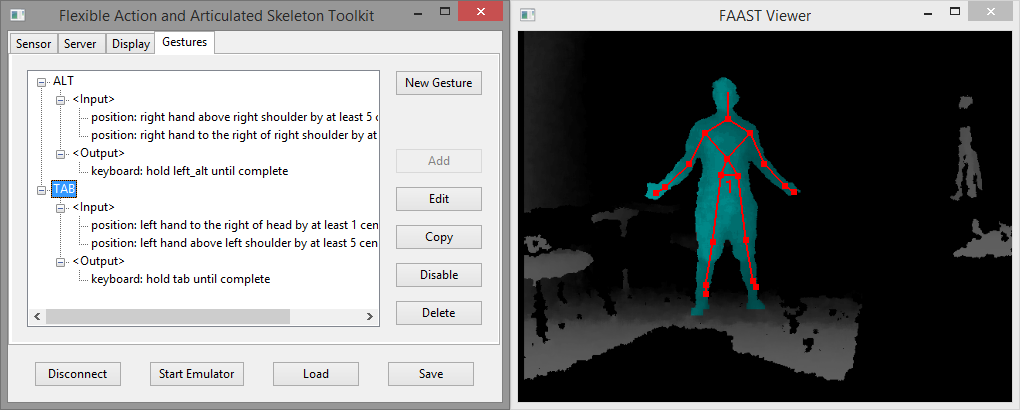
\includegraphics[width=0.8\textwidth]{faast}
\caption{FAAST \parencite{Suma:2013} provides atomic primitives that can be used to compose rules in plain English that map to mid-air gestures.}
\label{fig:faast}
\end{SCfigure}

\subsection{Discussion}

Above, tools that exemplify user interface paradigms for visually and textually authoring mid-air gestures have been presented (Table~\ref{tab:systems-summary}). For sensor-based gesturing, the standard paradigm used to represent gesture information appears to be projecting the sensor waveforms onto a graph. Graphs appear to work well as components that represent sensor- based gestures, allow experimentation with filters and gesture recognition methods, and support direct manipulation to some extent. User studies show that while the graphs alone may not allow developers to fully grasp the connection between movements and the waveform \parencite{Ashbrook:2010}, they have been deemed useful as part of a multimodal gesture representation \parencite{Zamborlin:2014}. Using hurdles as a visual markup language offers an intuitive and expressive medium for gesture authoring, but it is not able to depict fully 3-dimensional gestures. Using spherical control points may be more conducive to direct manipulation while still affording an expressive syntax, but no implementation of this paradigm exists for authoring mid-air gestures. Finally, timelines of frames may come in handy for visualizing dynamic gestures with many moving elements, such as in skeletal tracking; but, used in this fashion, they allow only visualization and not manipulation.

\begin{table}[ht]
\centering
\renewcommand{\arraystretch}{1.8}
\begin{tabular}{>{\raggedright\arraybackslash}m{.2\textwidth} >{\raggedright\arraybackslash}m{.2\textwidth} >{\raggedright\arraybackslash}m{.2\textwidth} >{\raggedright\arraybackslash}m{.28\textwidth}}
\textbf{System} &
\textbf{UI Paradigm} &
\textbf{Programming Approach} &
\textbf{Insights from Evaluation} \\
\hline
\textbf{Exemplar} \newline
\parencite{Hartmann:2007} &
Graphs &
Demonstration &
Increases engagement with sensor workings and limitations. \\
\textbf{MAGIC} \newline
\parencite{Ashbrook:2010} &
Graphs (multi-waveform) &
Demonstration &
Users unable to connect waveform to physical movements. Optional video is favored over graphs. \\
\textbf{GIDE} \newline
\parencite{Zamborlin:2014} &
Graphs (multi-waveform, with video) &
Demonstration &
Multimodal representation helps make sense of gesture data. \\
\textbf{EventHurdle} \newline
\parencite{Kim:2013} &
Visual markup language &
Declaration &
Easily understood. Supports “advanced” programming. \\
\textbf{Control Points} \newline
\parencite{Hoste:2013} &
Visual markup language &
Declaration and Demonstration &
Not implemented. \\
\textbf{Gesture Studio}\footnote{\href{http://www.gesturestudio.ca}{gesturestudio.ca}} &
Timeline &
Demonstration &
Not published. \\
\textbf{FAAST} \newline
\parencite{Suma:2013} &
Textual &
Declaration &
Widely adopted due to standalone, end-to-end implementation. \\
\hline
\end{tabular}
\caption{Summary of studies on systems that exemplify user interface paradigms for authoring mid-air gestures.}
\label{tab:systems-summary}
\end{table}
